\documentclass{article}[12pt,a4paper]
\usepackage{graphicx}
\usepackage{geometry}
\usepackage{tikz}
\usetikzlibrary{calc}

\begin{document}
\begin{titlepage}
    \begin{tikzpicture}[remember picture, overlay]
      \draw[line width = 1pt] ($(current page.north west) + (2em,-2em)$) rectangle ($(current page.south east) + (-2em,2em)$);
    \end{tikzpicture}

    \centering
    \vspace{-3em}
    {\Large\textbf{Mini Project Report}}\\
    \vspace{1.5em}
    On\\
    \vspace{1.5em}
    {\Huge \textbf{PASSWORD HASHING WITH}}\\
    \vspace{0.5em}
    {\Huge \textbf{SALT TECHNIQUE}}\\
    \vspace{2em}
    {\LARGE \bfseries Submitted by}\\
    \vspace{1em}
    {\Large \emph{\textbf{202IS027  Tridiv Kumar Rabha}}}\\
    {\Large \emph{\textbf{202IS020  Rubika Pradhan}\\
    }}
    \vspace{4em}
    {\Large Under the Guidance of}\\
    \vspace{2em}
    {\Large \textbf{Dr. P. Santhi Thilagam}}\\
    \vspace{2em}
    {\Large \textbf{Dept. of Computer Science \& Engineering,}}\\
    \vspace{1em}
    {\Large \textbf{NITK, Surathkal}}\\
    \vspace{2em}
    {\Large \textbf{Date of Submission: 24.5.2021}}\\
    \begin{figure}[!ht]
        \centering
        
\includegraphics{nitk-logo.png}
    \end{figure}
    {\Large \bfseries Department of Computer Science \& Engineering }\\
    \vspace{0.5em}
    {\Large \bfseries National Institute of Technology Karnataka, Surathkal.}\\
    \vspace{0.5em}
    {\Large \bfseries 2020-2021}
\end{titlepage}

\pagenumbering{roman}
\begin{center}
\section*{Abstract}
\end{center}

\addcontentsline{toc}{section}{Abstract}
\vspace{2em}
Keeping passwords in plain text is not a great solution because the attacker directly
owns all users’ passwords in plain text. No one, including website/database administrators, should have access to the user’s simple text password. Therefore in this project,
we would explain the main principles of secure storage (hash, salt, pepper, iteration) and highlight their importance for resisting password recovery methods. Finally, we would
proceed with a reliable hash function for secure storage.\\
\textbf{Hashing} passwords is the standard approach to storing passwords securely. A “Hash” is a one-way function that generates a representation of the password. A user’s password is taken, and using a key known to the site; the hash value is derived from the combination of both the password and the key, using a set algorithm. To verify a user’s password is correct, it is hashed, and the value compared with that stored on record each time they log in. Hashes are impossible to convert back into plain text, but you don’t need to convert them back to break them. Once you know that a particular string converts
to a specific hash, you know that any instance of that hash represents that string. It does not take much computational power to generate a table of hashes of combinations of letters, numbers and symbols. Once you have this store of hashes, you can then compare the hash you want to crack and see if it matches. Once you find a match, you know the
password. Exposing a hash can be made difficult by adding salt to it. Salts create unique passwords, even in the instance of two users choosing the same passwords. Salts help us mitigate hash table attacks by forcing attackers to re-compute them using the salts for each user. We cannot convert a hashed value into a password directly. Still, you can work out the password if you continually generate hashes from passwords until you find one that matches a so-called brute-force attack.

\newpage
\begin{center}
\section*{Declaration}
\end{center}

\addcontentsline{toc}{section}{Declaration}
\vspace{2em}
We solemnly declare that the project reports \textbf{“Password Hashing Using Salt Technique”} is based on our work carried out during our study under the supervision of \textbf{Dr. P. Santhi Thilagam}.
We assert the statements made and conclusions drawn as an outcome of our research work. We further certify that
\begin{itemize}
\item The work contained in the report is original and has been done by me under the general supervision of my supervisor.
\item The work has not been submitted to any other Institution for any other degree, diploma, a certificate in this university or the any other University of India or abroad.
\item We have followed the guidelines provided by the university in writing the report.
\item Whenever we have used materials (data, theoretical analysis, and text) from other sources, we have given due credit to them in the text of the report and given their details in the references.
\end{itemize}
\vspace{33em}
\textbf{Tridiv Kumar Rabha(202IS027)}\\
\textbf{Rubika Pradhan(202IS020)}
\newpage
\begin{center}
\section*{Certificate}    
\end{center}
\vspace{2em}
This is to certify that the report entitled \textbf{PASSWORD HASHING WITH SALT TECHNIQUE} submitted by \textbf{Tridiv Kumar Rabha} and \textbf{Rubika Pradhan} to the \textbf{NATIONAL INSTITUTE OF TECHNOLOGY KARNATAKA} in partial fulfillment of the requirements for the award of the Degree of Master of Technology in Computer Science and Information Security is a bonafide record of the project work carried out by them under my guidance and supervision.\\
This report in any form has not been submitted to any other University or Institute for any purpose.\\

\vspace{35em}
\textbf{Supervisor: Dr. P. Santhi Thilagam\\
Dep. Of Computer Science and Engineering\\
National Institute of Technology, Karnataka\\ 
Surathkal, Mangalore - 575025}\hspace{16em}\textbf{Date: 24th May, 2021}
\addcontentsline{toc}{section}{Cerificate}



\newpage
\tableofcontents
\thispagestyle{empty}
\newpage
\pagenumbering{arabic}

\section{Introduction}
Technology changes fast. Increasing the speed and power of computers can benefit both the engineers trying to build software systems and the attackers trying to exploit them. Some cryptographic software is not designed to scale with computing power. As explained earlier, the safety of the password depends on how fast the selected cryptographic hashing function can calculate the password hash. A fast function would execute faster when running in much more powerful hardware.\\
The salt is a pollutant to the raw data (here the password), producing two different hashes from the same data.  The salt is unique for each user and is composed of a random sequence.  It increases the chance that a password is unique and, therefore, a hash has never been used. 
The advantages of salt are multiple:
\begin{itemize}
    \item It is almost impossible to find hash directly on the internet if it is salted. However, the salt must be long enough and random.
    \item Rainbow tables do not work with salted hash.
    \item As said before, two users with the same password will not have the same hash if salt is used. After breaking a hash, password cracking software (hashcat, Johntheripper) looks to see if it is not present for another user.
\end{itemize}
bcrypt is a hash function created by Niels Provos and David Mazières. It is based on the Blowfish encryption algorithm and was presented at USENIX in 1999. 
Since this algorithm dates back to 1999, it has shown its robustness over time, where some algorithms like Argon2 only exist since 2015.
The hash computed by bcrypt has a predefined form:\\
\$2y\$11\$SXAXZyioy60hbnymeoJ9.ulscXwUFMhbvLaTxAt729tGusw.5AG4C
\begin{itemize}
    \item \textbf{Algorithm}: This one can take several versions depending on the version of bcrypt (\$2\$, \$2a\$, \$2x\$, \$2y\$ and \$2b\$)
    \item \textbf{The cost}: The number of iterations in the power of 2. For example, the iteration is 11, and the algorithm will do 211 iterations (2048 iterations).
    \item \textbf{Salt}: Instead of storing the salt in a dedicated column, it is directly stored in the final hash.
\item \textbf{The hashed password}
\end{itemize}

Since bcrypt stores the number of iterations, this makes it an adaptive function because it can increase the number of iterations, and therefore it is longer and longer. Despite its age and the evolution of computing power, this allows it to be still robust against brute force attacks. The following benchmark shows that it takes 23 days for hashcat to compute the totality of rockyou hashes.

Interestingly, the passwords azerty and matrix, being very weak passwords and present at the top of the list, were found during the short time (2 hours) that the software worked in the example. 
\newpage
\pagenumbering{arabic}

\section{Implementation}
\subsection{Technologies used}
\begin{itemize}
    \item Node JS
    \item MongoDB 
    \item Ejs
    \item Express JS
\end{itemize}
\subsection{Application Overview}
A user can register with a username and password in our application. The authenticated user can also see his profile details in our application. We have stored the registration credentials in a database. Passwords provided by the users are stored in hashed form with salting. 
\begin{figure}[hbt!]
        \centering
        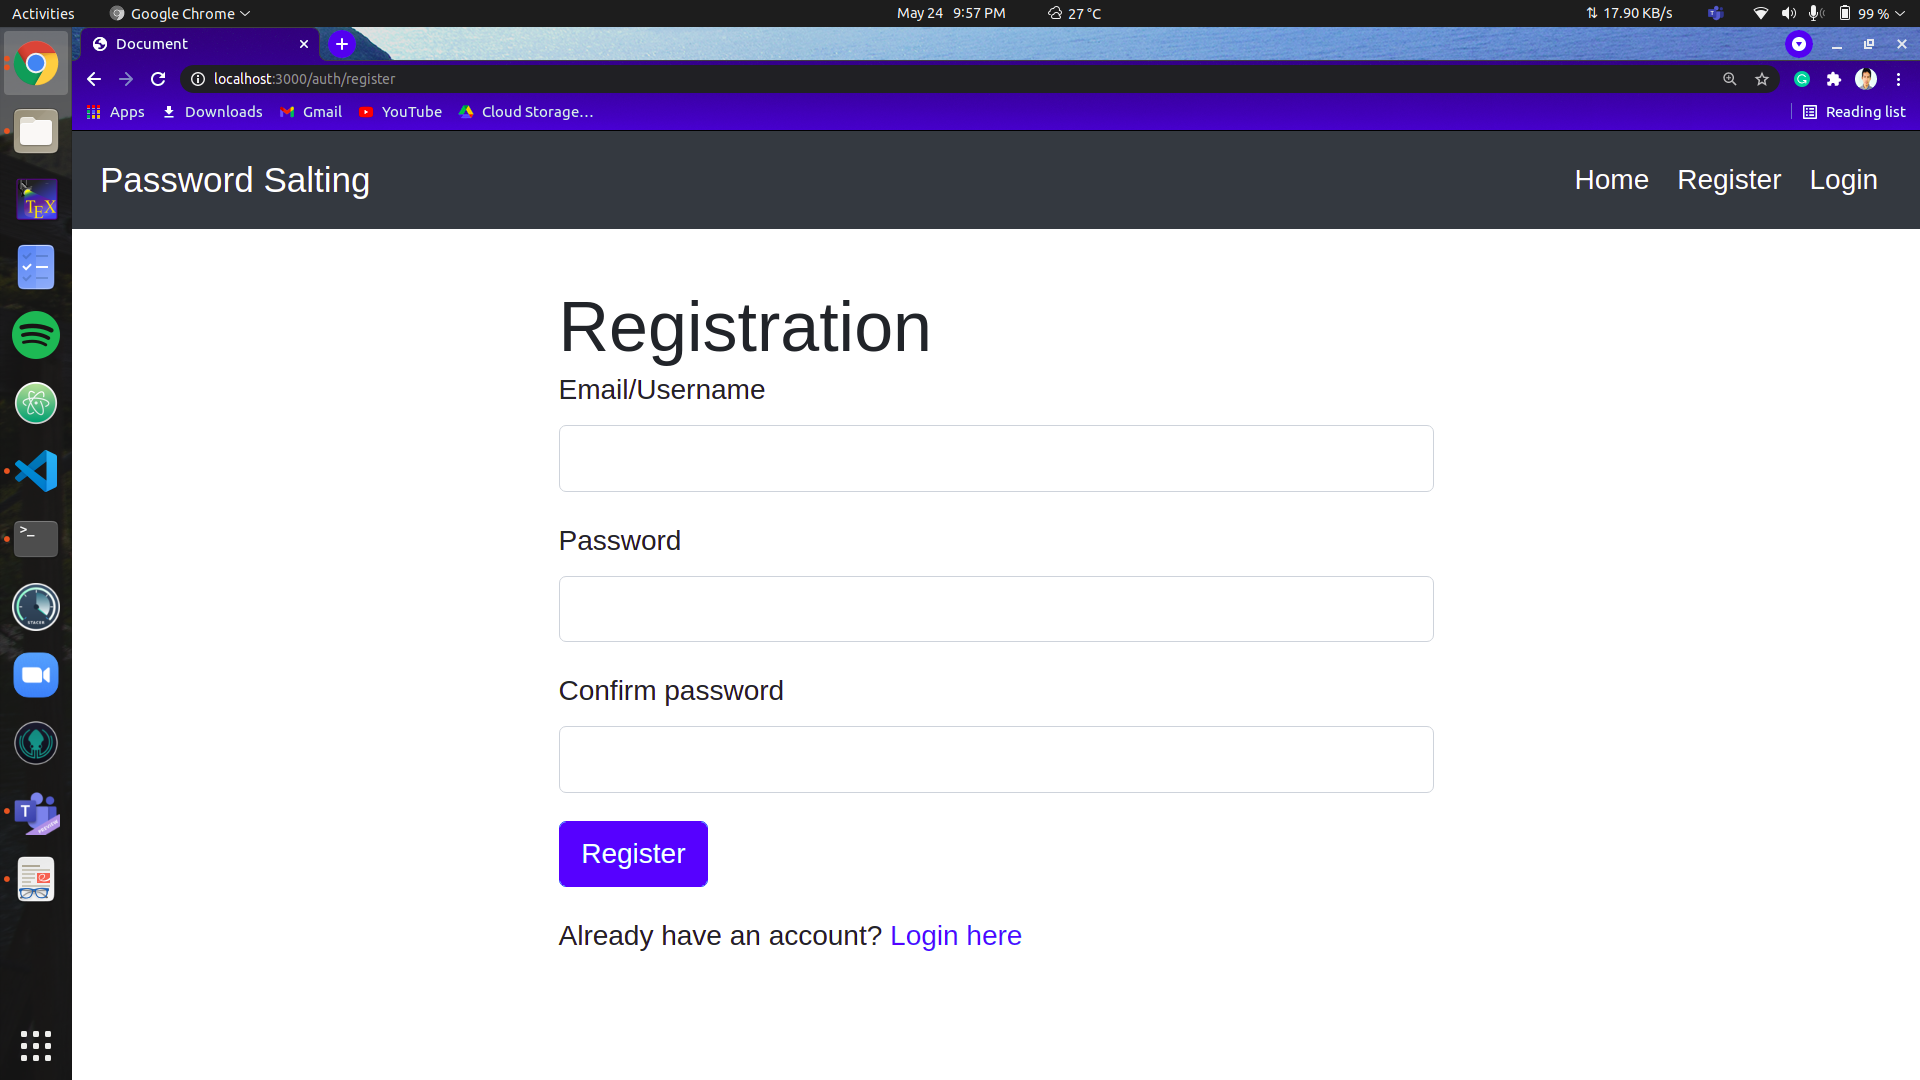
\includegraphics[scale=0.2]{regstn.png}
        \caption{Registration page}
\end{figure}
\newpage
\begin{figure}[hbt!]
        \centering
        \includegraphics[scale=0.2]{login.png}
        \caption{Login page}
\end{figure}
\begin{figure}[hbt!]
        \centering
        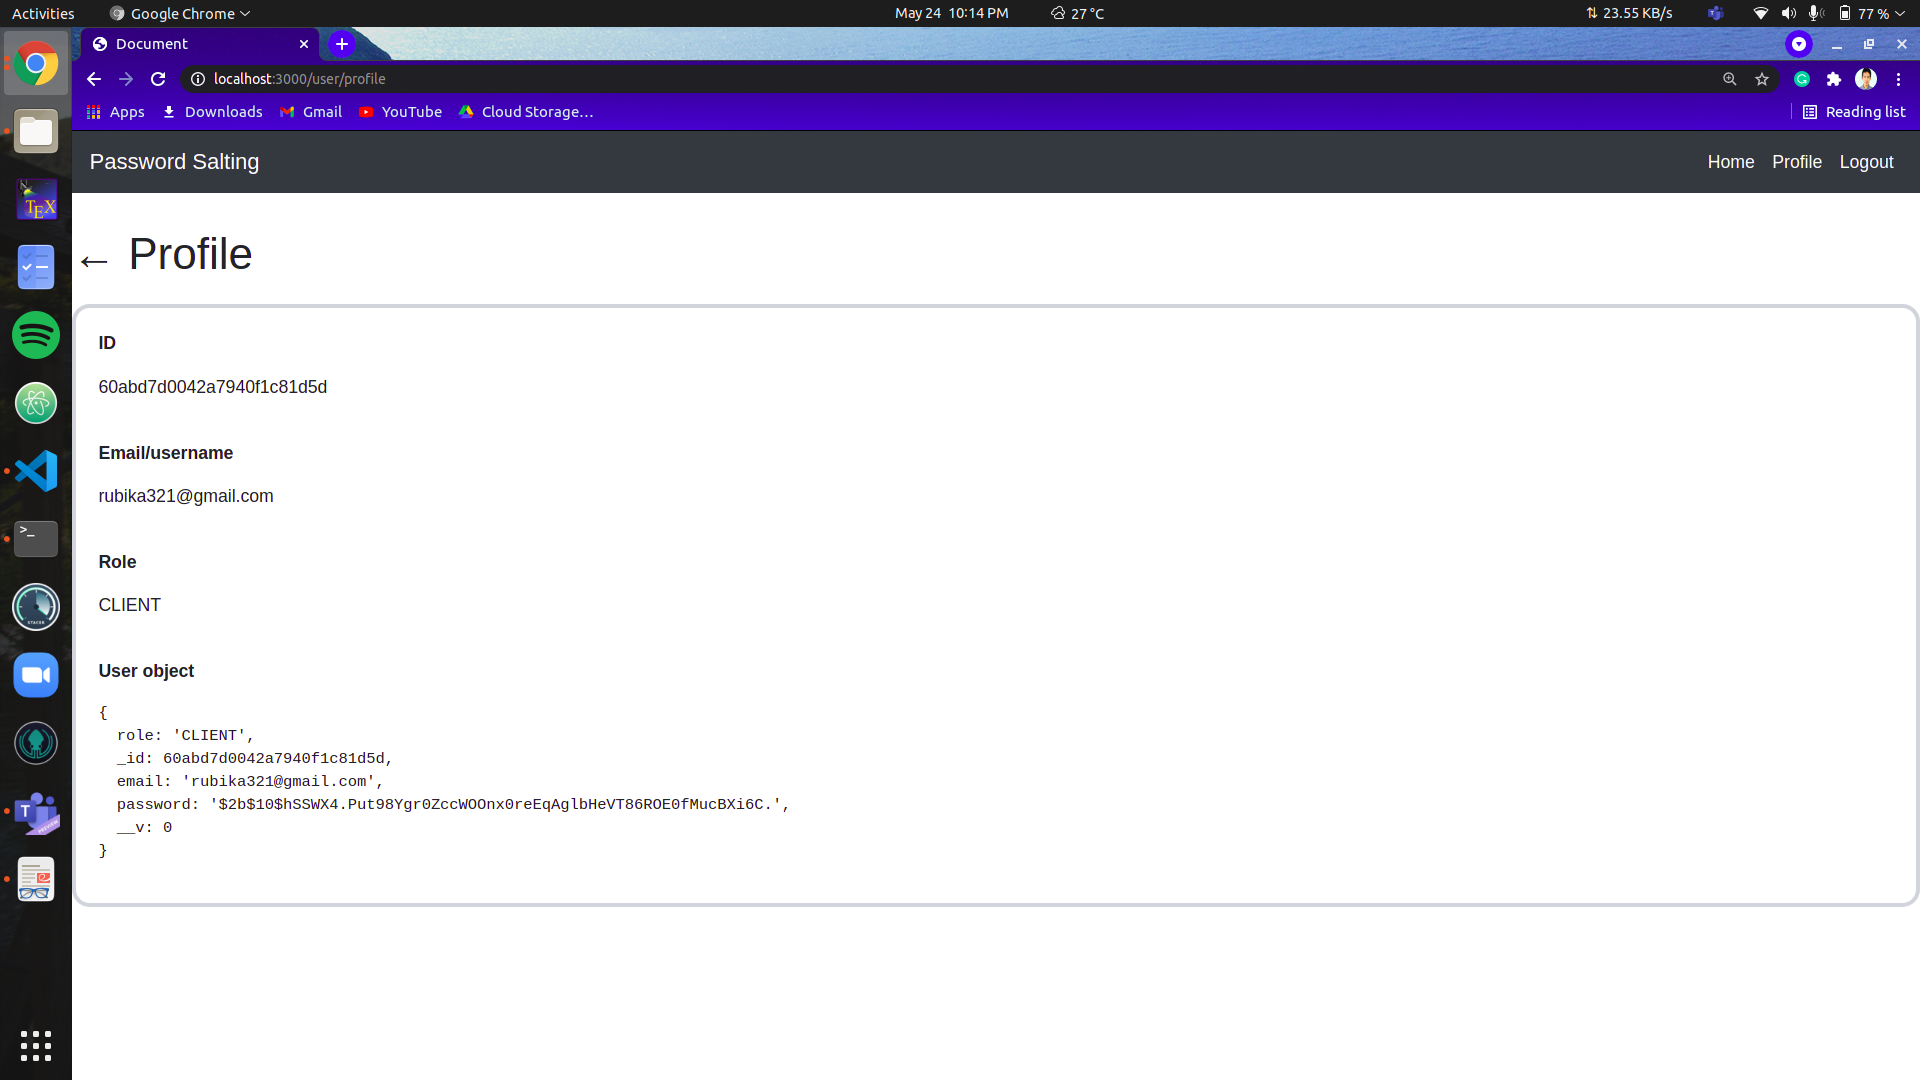
\includegraphics[scale=0.2]{profile.png}
        \caption{Profile page}
\end{figure}
\newpage
\subsection{Rainbow table attack}
Rainbow tables are a subject that deserves an article on its own. Quickly, it’s a data structure that allows retrieving passwords with a good storage/time compromise. This structure has a list of pre-calculated hashes and makes it possible to retrieve a hash in an acceptable time. \\
Many rainbow tables are available online and also we can create on our local system.
We created a rainbow table using the md5 function and then found the hash value of the password we want to find in the rainbow table. We were successful in getting the plain text of the hashed password from the rainbow table. We then tried to find the salted hash of the password in our rainbow table, but we could not. Therefore, it is proved that password salting is not susceptible to rainbow table attacks.
\begin{figure}[hbt!]
        \centering
        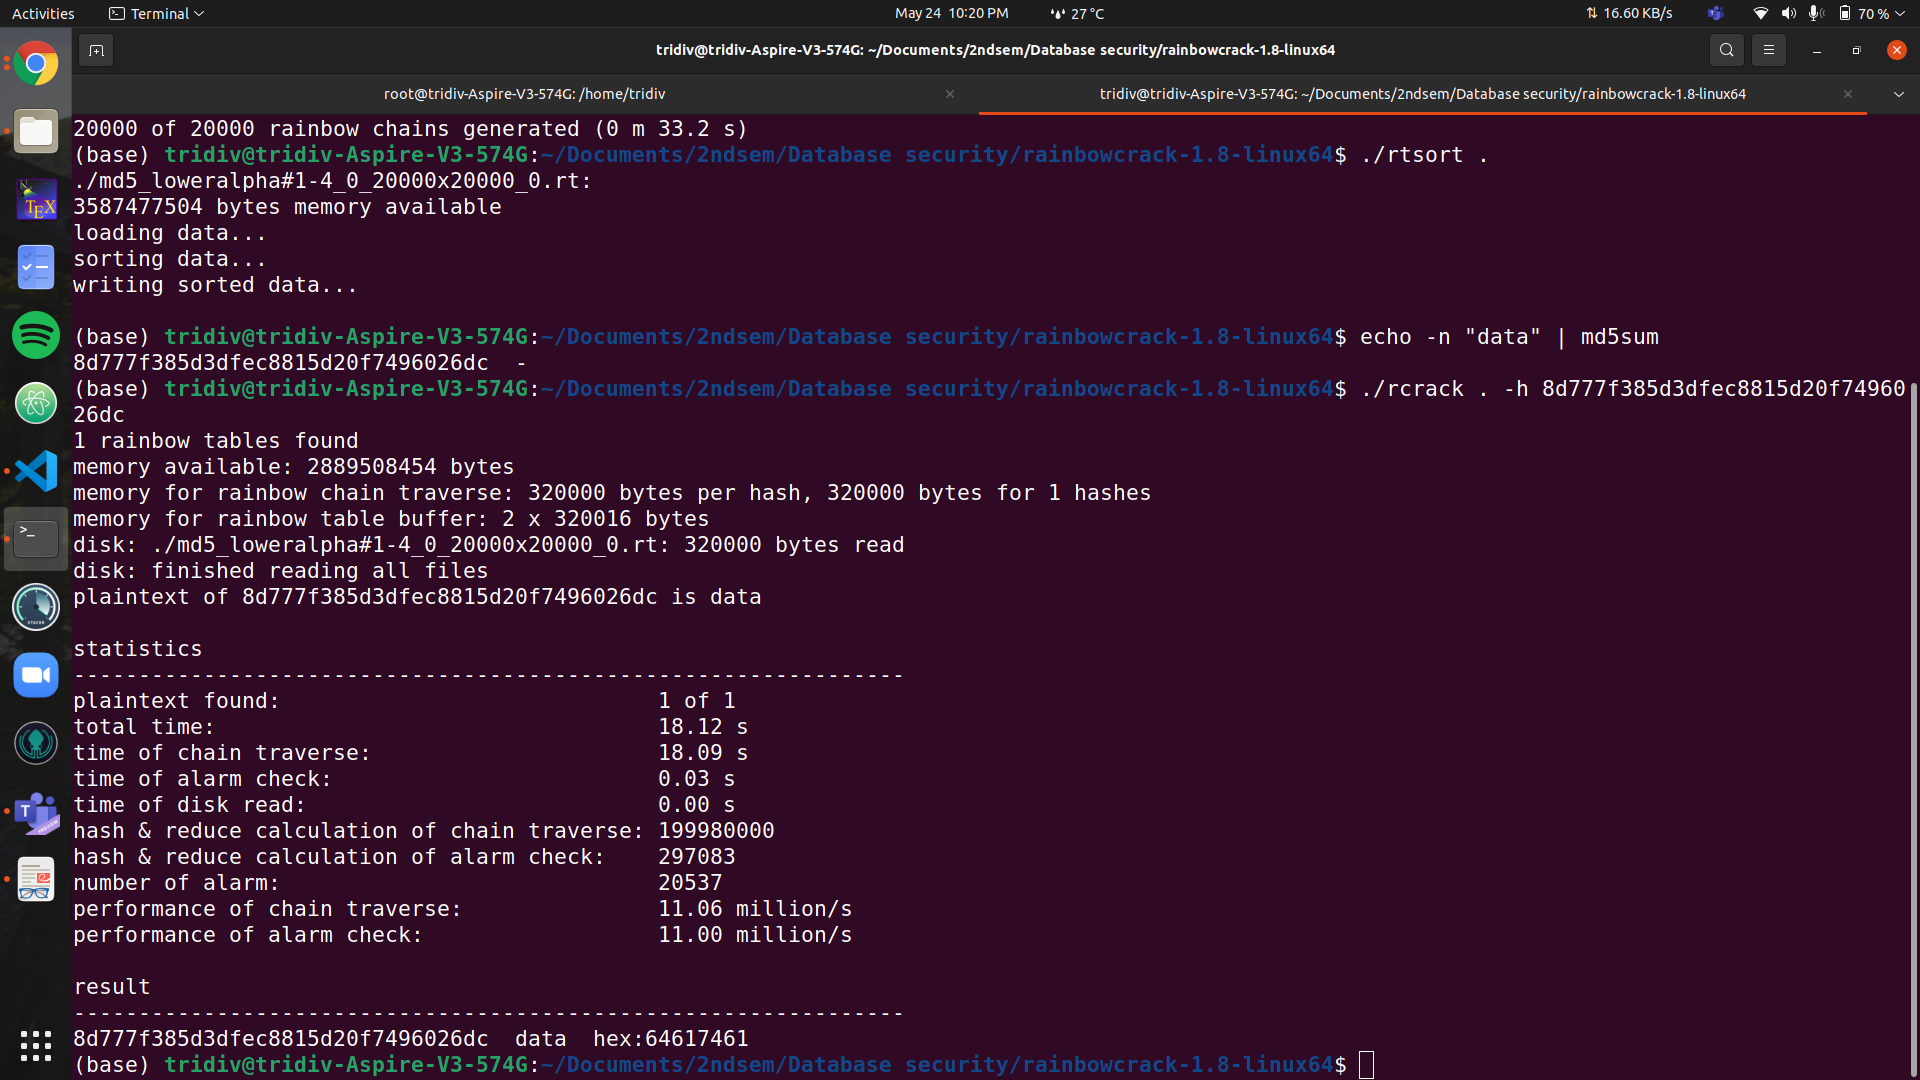
\includegraphics[scale=0.2]{rainbow.png}
        \caption{Rainbow table attack}
\end{figure}
\newpage
\section{Conclusion}
Hashing passwords alone is
not enough. Hackers are aware of many hashing algorithms, and they keep lists, called rainbow tables, of common hashes of common passwords. They have got most if not all the hashes for “pass123″ and similarly common passwords. So, if any one of those hashes appears in the list, the entire hashing scheme becomes known, and all the other more unusual passwords become much more easily compromised as well.

That’s where salting comes in. You can’t force users to come up with good passwords on their own – there’s always going to be someone trying to get away with “pass123.” What you can do is make the password better on the machine level. You can add some extra bits to it, called a “salt.” For example, “pass123″ becomes “8Ytu9j06pass123.” Much better! You do have to store the salt in your database somewhere, because your user does not have that part memorized. If your system is compromised, that means the salt gets compromised as well. However, the benefit is this: when you run that salted password through a hashing algorithm, it produces a different hash than the one produced by “pass123″ on its own. That means that rainbow tables have to contain thousands more entries for each common password plus all the salt possibilities for each common password, making them a much less effective tool for password cracking.
Therefore, if you have to store passwords, always make sure they’re hashed and salted. You should still have everyone change their passwords if you get hacked, but this method should give you a bit more time and security.
\begin{thebibliography}{1}
\addcontentsline{toc}{section}{References}
    
\bibitem{ref1} Diksha.S.Borde, Poonam.A.Hebare, Priyanka.D.Dhanedhar, ``Overview Of Web Password Hashing Using Salt Technique". 
\bibitem{ref2} Praveen Gauravaram,``Security Analysis of salt||password Hashes"
\bibitem{ref3} https://en.wikipedia.org/wiki/Bcrypt
\bibitem{ref4} https://www.npmjs.com/package/bcrypt
\bibitem{ref5} https://www.educative.io/edpresso/what-is-hashing
\end{thebibliography}
\end{document}
